\begin{frame}{Applications Physiques}{Equations d'ADR}
\begin{center}
    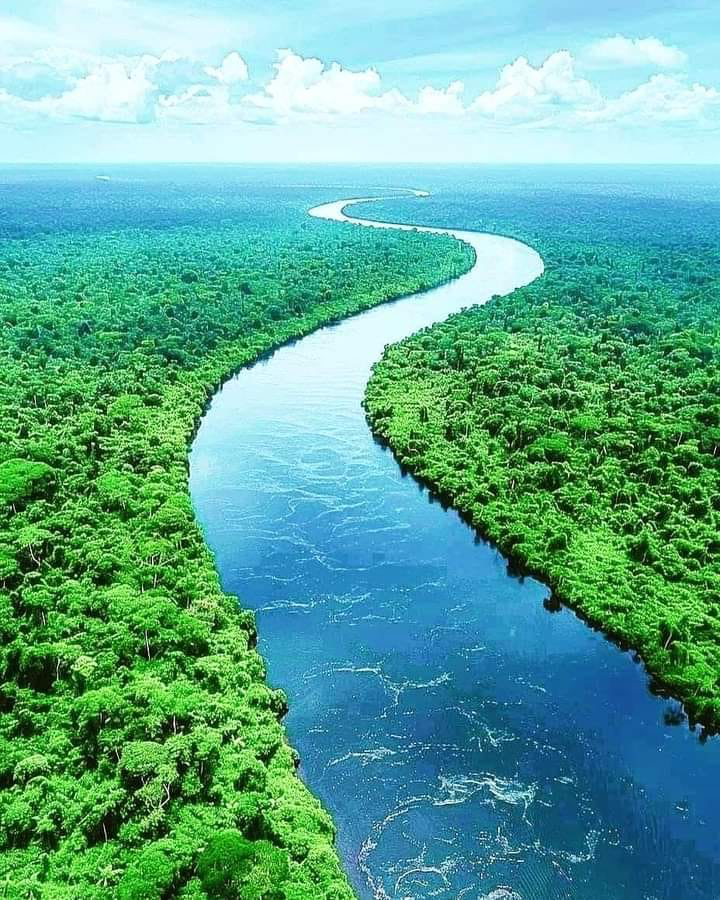
\includegraphics[height=0.4\textheight]{medias/1_/rio_amazonas.png}\hfill
    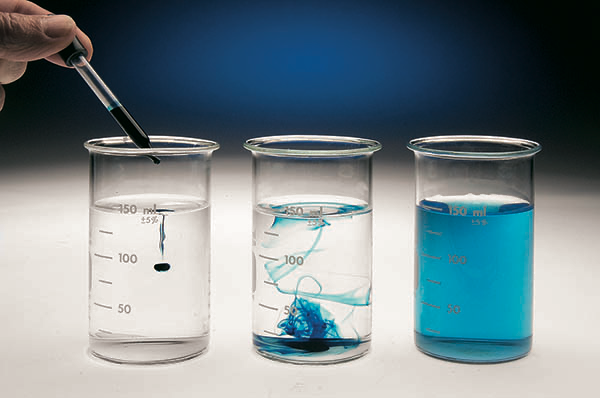
\includegraphics[height=0.4\textheight]{medias/1_/ink_diffusion.png}\hfill
    
\includegraphics[height=0.4\textheight]{medias/1_/chemical_reaction.png}
\end{center}
\pause
    \begin{equation}
        \begin{cases}
            \partial_t u(x,t) = 
                \overbrace{\underbrace{A u}_{c \partial_x u}}^{\text{Advection}}+ 
                \overbrace{\underbrace{D u}_{\partial_x(\eta \partial_x u)}}^{\text{Diffusion}}+ 
                \overbrace{\underbrace{R(u)}_{\text{Non-lin.}}}^{\text{Réaction}},\\[4pt]
            u(x,0)=u_0.
        \end{cases}
    \end{equation}

\end{frame}